%\documentclass[paper=a4,abstract=on,cleardoublepage=empty,numbers=noenddot,toc=bib,12pt,appendixprefix=true]{scrreprt}
\documentclass[%
    a4paper,              % DIN A4
    style=screen,          % print: enables twoside, print colors, and BCOR=15mm
    bibliography=totoc,   % bibliography gets unnumbered entry
    nexus,                % corporate design font
    lnum,                 % use "Versalziffern" instead of "Mediaevalziffern"
    extramargin,          % override corporate design margin to give more space for one-column text
]{tubsbook}

%\usepackage[T1]{fontenc}
\usepackage[utf8]{inputenc}

\usepackage{pgfplots}
%\usepackage{microtype}
\usepackage{xcolor}
    \definecolor{medium-blue}{rgb}{0,0,0.5}
\usepackage{hyperref}
\usepackage{amsmath}
\usepackage{amsthm}
\usepackage{mathtools}
\usepackage[nameinlink]{cleveref}
    \newtheorem{theorem}{Theorem}
    \newtheorem{corollary}{Corollary}
    \theoremstyle{definition}
    \newtheorem{definition}{Definition}
    \newtheorem{lemma}{Lemma}
\usepackage{amsfonts}
\usepackage{todonotes}
\usepackage{tikz}
    \newcommand{\B}{1.36207}

\tikzset{tight/.style={inner sep=1pt}}
\tikzset{bracket/.style={inner sep=10pt,draw=gray,decorate,decoration={brace,amplitude=5pt}}}
\tikzset{filled/.style={fill=black!30!white}}
\tikzset{filled2/.style={fill=black!15!white}}

%\newcommand\hatshape[3][]{
%    \pgfmathsetmacro{\r}{sqrt((#2)/pi)}
%    \pgfmathsetmacro{\s}{sqrt((#3)/pi)}
%
%    \coordinate (top) at (0,{(\r/(sqrt(2)-1)});
%    \coordinate (right) at ({(\r/(sqrt(2)-1)},0);
%    \coordinate (left) at ({(-\r/(sqrt(2)-1)},0);
%
%    \coordinate (leftcenter) at ($({-(\r-\s)/(sqrt(2)-1)},0)+(0,\s)$);
%    \coordinate (leftbottom) at ($(leftcenter)+(-90:\s)$);
%    \coordinate (lefttop) at ($(leftcenter)+(-225:\s)$);
%
%    \coordinate (rightcenter) at ($({(\r-\s)/(sqrt(2)-1)},0)+(0,\s)$);
%    \coordinate (rightbottom) at ($(rightcenter)+(-90:\s)$);
%    \coordinate (righttop) at ($(rightcenter)+(45:\s)$);
%
%    \coordinate (midcenter) at (0,\r);
%
%    \draw[#1] (rightbottom) arc (-90:45:\s) -- (top) -- (lefttop) arc (-225:-90:\s) -- cycle;
%}

\newcommand\hatshape[5][]{
    \pgfmathsetmacro{\r}{sqrt((#2)/pi)}
    \pgfmathsetmacro{\s}{sqrt((#3)/pi)}
    \pgfmathsetmacro{\a}{(#4)}
    \pgfmathsetmacro{\b}{(#5)}

    \coordinate (top) at ({cos((90+(\a-\b)/2))*(\r/cos((\a+\b)/2))},{sin((90+(\a-\b)/2))*(\r/cos((\a+\b)/2)});
    \coordinate (left) at ({-\r/tan(\a/2)},-\r);
    \coordinate (right) at ({\r/tan(\b/2)},-\r);

    \coordinate (leftcenter) at ($(left)+({\s/tan(\a/2)},\s)$);
    \coordinate (leftbottom) at ($(leftcenter)+(-90:\s)$);
    \coordinate (lefttop) at ($(leftcenter)+({-270+\a}:\s)$);

    \coordinate (rightcenter) at ($(right)+({-\s/tan(\b/2)},\s)$);
    \coordinate (rightbottom) at ($(rightcenter)+(-90:\s)$);
    \coordinate (righttop) at ($(rightcenter)+({90-\b}:\s)$);

    \coordinate (topcenter) at ($(top)-({cos((90+(\a-\b)/2))*(\s/cos((\a+\b)/2))},{sin((90+(\a-\b)/2))*(\s/cos((\a+\b)/2)})$);
    \coordinate (topleft) at ($(topcenter)+({-270+\a}:\s)$);
    \coordinate (topright) at ($(topcenter)+({90-\b}:\s)$);

    \coordinate (midcenter) at (0,0);

    %\draw[#1] (right) -- (top) -- (left) -- cycle;
    \draw[#1] (rightbottom) arc (-90:{90-\b}:\s) -- (topright) arc ({90-\b}:{90+\a}:\s) -- (lefttop) arc ({-270+\a}:-90:\s) -- cycle;
}
\newcommand\gemshape[3][]{
    \pgfmathsetmacro{\r}{sqrt((#2)/pi)}
    \pgfmathsetmacro{\s}{sqrt((#3)/pi)}
    \pgfmathsetmacro{\l}{0.85955*sqrt(#3)}
    \pgfmathsetmacro{\ll}{0.7654*\l}
    \pgfmathsetmacro{\a}{45}
    \pgfmathsetmacro{\b}{45}

    \coordinate (top) at ({cos((90+(\a-\b)/2))*(\r/cos((\a+\b)/2))},{sin((90+(\a-\b)/2))*(\r/cos((\a+\b)/2)});
    \coordinate (left) at ({-\r/tan(\a/2)},-\r);
    \coordinate (right) at ({\r/tan(\b/2)},-\r);

    \coordinate (leftcenter) at ($(left)+({\s/tan(\a/2)},\s)$);
    \coordinate (lefttop) at ($(left)+(45:\l)$);
    \coordinate (leftmid) at ($(left)+(22.5:\ll)$);
    \coordinate (leftbottom) at ($(left)+(0:\l)$);

    \coordinate (rightcenter) at ($(right)+({-\s/tan(\b/2)},\s)$);
    \coordinate (righttop) at ($(right)+(135:\l)$);
    \coordinate (rightmid) at ($(right)+(157.5:\ll)$);
    \coordinate (rightbottom) at ($(right)+(180:\l)$);

    %\coordinate (topcenter) at ($(top)-({cos((90+(\a-\b)/2))*(\s/cos((\a+\b)/2))},{sin((90+(\a-\b)/2))*(\s/cos((\a+\b)/2)})$);
    %\coordinate (topleft) at ($(topcenter)+({-270+\a}:\s)$);
    %\coordinate (topright) at ($(topcenter)+({90-\b}:\s)$);

    \coordinate (midcenter) at (0,0);

    \draw[#1] (top) -- (righttop) -- (rightmid) -- (rightbottom) -- (leftbottom) -- (leftmid) -- (lefttop) -- cycle;
    %\draw[#1] (rightbottom) arc (-90:{90-\b}:\s) -- (top) arc ({-270+\a}:-90:\s) -- cycle;
}

\newcommand\hatsinsquare[1]{
    \draw (0,0) rectangle (\B,\B);

    \pgfmathparse{\B-sqrt((1-(#1))/pi)}
    \begin{scope}[shift={(\pgfmathresult,\pgfmathresult)}]
        \begin{scope}[rotate=-45]
            \pgfmathsetmacro{\hata}{1-(#1)}
            \pgfmathsetmacro{\hatb}{1-2*(#1)}
            \hatshape[filled2]{\hata}{\hatb}{45}{45}
            \node at (midcenter) {\hata};
        \end{scope}
    \end{scope}

    \def\comparg{#1}
    \if\comparg0\else
        \pgfmathparse{(sqrt((#1)/pi)}
        \begin{scope}[shift={(\pgfmathresult,\pgfmathresult)}]
            \begin{scope}[rotate=-225]
                \hatshape[filled2]{#1}{0}{45}{45}
                \node at (midcenter) {#1};
            \end{scope}
        \end{scope}
    \fi
}

% alpha, beta, incircle-area of right hat, rounding
\newcommand\hatsinhat[4]{
    \pgfmathsetmacro{\a}{(#1)}
    \pgfmathsetmacro{\b}{(#2)}
    \pgfmathsetmacro{\x}{(#3)}
    \pgfmathsetmacro{\round}{(#4)}
    \pgfmathsetmacro{\f}{(cos(\b/2)^2*sec(\a/2+\b/2)^2*(1-sin(\a)))}
    \pgfmathsetmacro{\g}{(cos(\a/2)^2*sec(\a/2+\b/2)^2*(1-sin(\b)))}

    \hatshape{1}{\round}{\a}{\b}

    \def\comparg{\x}
    \if\comparg0\else
        \pgfmathparse{sqrt(1/pi)/tan(\b/2)-sqrt(((\x))/pi)/tan(\b/2)}
        \begin{scope}[shift={(\pgfmathresult,0)}]
            \pgfmathparse{sqrt(1/pi)-sqrt(\x/pi)}
            \begin{scope}[shift={(0,-\pgfmathresult)}]
                \pgfmathsetmacro{\hata}{\x}
                \pgfmathsetmacro{\hatb}{max(\round,\x-\g*(1-\x)/(\f)))}
                \hatshape[filled2]{\hata}{\hatb}{90}{\b}
                \node at (midcenter) {\hata};
            \end{scope}
        \end{scope}
    \fi

    \def\comparg{\x}
    \if\comparg1\else
        \pgfmathparse{sqrt(1/pi)/tan(\a/2)-sqrt(((1-\x))/pi)/tan(\a/2)}
        \begin{scope}[shift={(-\pgfmathresult,0)}]
            \pgfmathparse{sqrt(1/pi)-sqrt((1-\x)/pi)}
            \begin{scope}[shift={(0,-\pgfmathresult)}]
                \pgfmathsetmacro{\hata}{1-\x}
                \pgfmathsetmacro{\hatb}{\round}
                \pgfmathsetmacro{\hatb}{max(\round,(1-\x)-\f*(\x)/(\g)))}
                \hatshape[filled2]{\hata}{\hatb}{\a}{90}
                \node at (midcenter) {\hata};
            \end{scope}
        \end{scope}
    \fi
}

% incircle-area of right hat, rounding
\newcommand\gemsingem[2]{
    \pgfmathsetmacro{\a}{45}
    \pgfmathsetmacro{\b}{45}
    \pgfmathsetmacro{\x}{(#1)}
    \pgfmathsetmacro{\round}{(#2)}
    \pgfmathsetmacro{\f}{(cos(\b/2)^2*sec(\a/2+\b/2)^2*(1-sin(\a)))}
    \pgfmathsetmacro{\g}{(cos(\a/2)^2*sec(\a/2+\b/2)^2*(1-sin(\b)))}

    \gemshape{1}{\round}

    \def\comparg{\x}
    \if\comparg0\else
        \pgfmathparse{sqrt(1/pi)/tan(\b/2)-sqrt(((\x))/pi)/tan(\b/2)}
        \begin{scope}[shift={(\pgfmathresult,0)}]
            \pgfmathparse{sqrt(1/pi)-sqrt(\x/pi)}
            \begin{scope}[shift={(0,-\pgfmathresult)},rotate=135]
                \pgfmathsetmacro{\hata}{\x}
                \pgfmathsetmacro{\hatb}{max(\round,\x-\g*(1-\x)/(\f)))}
                \gemshape[filled2]{\hata}{\hatb}
                \node at (midcenter) {\hata};
            \end{scope}
        \end{scope}
    \fi

    \def\comparg{\x}
    \if\comparg1\else
        \pgfmathparse{sqrt(1/pi)/tan(\a/2)-sqrt(((1-\x))/pi)/tan(\a/2)}
        \begin{scope}[shift={(-\pgfmathresult,0)}]
            \pgfmathparse{sqrt(1/pi)-sqrt((1-\x)/pi)}
            \begin{scope}[shift={(0,-\pgfmathresult)}]
                \pgfmathparse{\x < 0.1715 ? 0 : -135}
                \begin{scope}[rotate=\pgfmathresult]
                    \pgfmathsetmacro{\hata}{1-\x}
                    \pgfmathsetmacro{\hatb}{\round}
                    \pgfmathsetmacro{\hatb}{\x < 1/3 ? (1-\x) : max(\round,(1-\x)-\f*(\x)/(\g))}
                    \pgfmathsetmacro{\fillstyle}{\x < 1/3 ? "filled" : "filled2"}
                    \gemshape[\fillstyle]{\hata}{\hatb}
                    \node at (midcenter) {\hata};
                \end{scope}
            \end{scope}
        \end{scope}
    \fi
}

\newcommand\hatconstruction{
    \hatshape[draw=none]{1}{0.3}

    \draw[dashed] (rightcenter) circle(\s);
    \draw[dashed] (leftcenter) circle(\s);
    \draw[dashed] (midcenter) circle(\r);
    \draw[dashed] (right) -- (top) -- (left) -- cycle;

    \draw[tight] (rightcenter) -- node[below left] {$s$} ++(-45:\s) -- node[below right] {$s$} ++(45:\s) coordinate (rightright) {} -- node[right] {$s$} ++(-90:\s) -- node[above] {$s$} (right);
    \draw[thick,orange] (rightright) -- node[sloped,above] {$s\sqrt{2}$} (right);

    \draw[tight] (leftcenter) -- node[above] {$s$} ++(180:\s) -- node[left] {$s$} ++(-90:\s) coordinate (leftleft) {} -- node[below left] {$s$} ++(135:\s) -- node[below right] {$s$} (left);
    \draw[thick,orange] (leftleft) -- node[below] {$s\sqrt{2}$} (left);

    \draw[thick,left,blue] (0,0) -- node {$r$} (midcenter) -- node {$r\sqrt{2}$} (top);
    \draw (midcenter) -- node[below right] {$r$} +(45:\r) -- node[above right] {$r$} (top);
    \draw[thick,red] (left) -- node[sloped,above] {$(r+r\sqrt{2})\sqrt{2}$} (top);

    \coordinate (leftofleft) at ($(left)+(180:5pt)$);
    \coordinate (belowleft) at ($(left)-(90:5pt)$);
    \coordinate (farbelowleft) at ($(left)-(90:10pt)$);
    \coordinate (abovetop) at ($(top)+(45:5pt)$);
    \coordinate (farabovetop) at ($(top)+(45:10pt)$);
    \coordinate (faraboveright) at ($(right)+(45:10pt)$);
    \coordinate (aboverightright) at ($(rightright)+(45:5pt)$);
    \coordinate (leftend) at ($(leftleft)-(90:5pt)$);
    \coordinate (rightend) at ($(rightright)-(90:5pt)$);
    \coordinate (totheright) at ($(rightcenter)+(0:\s)$);
    \coordinate (rightend) at ($(totheright)-(90:5pt)$);

    \draw[bracket] (leftofleft) -- node[left] {$h(a)$} (leftofleft |- top);
    \draw[bracket] (rightend |- belowleft) -- node[below] {$w(a,b)$} (leftend |- belowleft);
    \draw[bracket] (rightend |- farbelowleft) -- node[below] {$w'(a,b)$} (left |- farbelowleft);
    \draw[bracket] (abovetop) -- node[above,sloped] {$d(a,b)$} (aboverightright);
    \draw[bracket] (farabovetop) -- node[above,sloped] {$d'(a)$} (faraboveright);
}

    \usetikzlibrary{calc}
    \usetikzlibrary{arrows}
\usepackage{graphicx}
    \graphicspath{{images/}}
\usepackage{algorithm}
\usepackage{algpseudocode}
    \renewcommand{\algorithmicrequire}{\textbf{Input:}}
    \renewcommand{\algorithmicensure}{\textbf{Output:}}
\usepackage{chngcntr}
    \counterwithout{equation}{chapter}

\newcommand{\C}{\mathbb{C}}
\newcommand{\s}{\sqrt{2}}
\DeclareMathOperator{\mysum}{sum}
\DeclareMathOperator*{\argmin}{arg\,min}


\usepackage[english]{babel} % hyphenation

\hypersetup{
    colorlinks, linkcolor={medium-blue},
    citecolor={medium-blue}, urlcolor={medium-blue}
}

\newcommand\defaulta{30}
\newcommand\defaultb{40}
\newcommand\defaultr{0.2}
\newcommand\defaultx{0.6}

%\titlehead{
%    \begin{center}
%        \includegraphics[width=0.5\textwidth]{square_example.png}
%    \end{center}
%}

\subject{Master's Thesis}
\title{Algorithms\\for Circle Packing}
\author{\sffamily\LARGE Sebastian Morr}
\date{\large June 2, 2016}
\publishers{\textbf{Institute of Operating Systems and Computer Networks\\Prof.\,Dr.\,Sándor\,Fekete}\\
\vspace*{2em}
Supervisors:\\
Dr.\,Christian\,Scheffer\\
Jan-Marc\,Reinhardt,\,M.\,Sc.}

\begin{document}
\frontmatter % roman page numbering

\maketitle
\cleardoublepage

% statement of originality
\thispagestyle{plain} % no header
\vspace*{7cm}
\centerline{\bfseries Statement of Originality}
\vspace*{1em}
\noindent
This thesis has been performed independently with the support of my supervisors.
To the best of the author's knowledge, this thesis contains no material previously
published or written by another person except where due reference is made in the text.

\par
  \bigskip\noindent Braunschweig, June 2, 2016 \par
  \vspace*{10mm}
  \hfill\hrulefill
\cleardoublepage

% abstract
\thispagestyle{plain} % no header
\centerline{\bfseries Abstract}
\vspace*{1em}
\noindent
Very abstract indeed.
\cleardoublepage

% include Aufgabenstellung pdf
%\includepdf[pages=-]{aufgabenstellung/Aufgabenstellung}
%\cleardoublepage

\section*{Acknowledgments}

I would like to thank the following people for their support in the creation of this thesis:

\section*{Colophon}

This document was created using \LaTeXe\ by Leslie Lamport and contributors, and \KOMAScript\ by Frank Neukam, Markus Kohm, and Axel Kielhorn. The figures were created using PGFPlots by Christian Feuersänger and Ti\textit{k}Z by Till Tantau. The text is set in the Latin Modern font family by Bogusław Jackowski, Janusz M. Nowacki and Marcin Woliński, the monospaced font is \texttt{Bera Mono}, based on Bitstream Vera.

\cleardoublepage
\setcounter{tocdepth}{2}

\tableofcontents
\cleardoublepage

%\listoffigures
%\cleardoublepage
%
%\listoftables
%\cleardoublepage

\mainmatter % arabic numbering

\chapter{Introduction}

\begin{figure}[htbp!]
    \centering

    \begin{tikzpicture}[scale=2.5]
        \squareworstcase
    \end{tikzpicture}

    \caption{Worst-case instance for packing density?}
    \label{fig:worst-case}
\end{figure}

Consider the circle packing shown in \Cref{fig:worst-case}. For these two circles, the surrounding square is the smallest one in which the circles can be packed. Originally, we considered the following problem: Does this instance constitute the worst case in terms of packing density, or is there a set of circles with the same combined area that cannot be packed into this square? Put differently, can all other sets of circles with the same combined area as these two
(like the one in \Cref{fig:big-question})
be packed into this specific square?
We will give a constructive proof that this is indeed the case.

\begin{figure}[htbp!]
    \centering

    \begin{tikzpicture}[scale=2.5]
        \bigquestion
    \end{tikzpicture}

    \caption{Can these circles be packed?}
    \label{fig:big-question}
\end{figure}

\chapter{Preliminaries}

%\section{Circle instances}

We start off with some definitions which make our life easier when talking about circles and circle instances:

\begin{definition}
    For each $0 \le a$, an \emph{$a$-circle} is a circle with an area of $a$.
\end{definition}

\begin{definition}
    A \emph{circle instance} is a multiset of non-negative real numbers, which define the circles' areas. Addition of circle instances is defined like on multisets.
\end{definition}

\begin{definition}
    For a circle instance $A$, $\mysum(A)$ is the combined area of the instance's circles.
\end{definition}

\begin{definition}
    $\C$ is the set of all circle instances. $\C(a)$ consist of exactly those circle instances with a combined area of at most $a$. Finally, $\C(a,b)$ consists of exactly those circle instances $A \in \C(a)$, for which each circle in $A$ has an area of at least $b$.
\end{definition}

\chapter{Common techniques}

\section{Greedy splitting}

The core idea of the proposed packing algorithms is to repeatedly split the set of input circles into groups. The method which performs this splitting resembles a greedy scheduling algorithm. It is going to be important for the packing algorithm that the ratio of the groups' sizes is close to certain factors.

The algorithm, \textsc{Split}, takes two parameters: The first is an arbitrary circle instance $C$. The second is a tuple of positive factors, which determines which percentages of $C$'s total area should go into the respective groups. For example, if we wanted to split $C$ into equally sized halves, we could choose the tuple $(1,1)$, and if we wanted to split $C$ into four groups with the proportions 1:1:3:3, we could use $(1,1,3,3)$. We call this tuple the \emph{split key}:

\begin{definition}
    A \emph{split key} is a tuple of at least two positive real numbers.
\end{definition}

Of course, it will not always be possible to achieve this desired ratio exactly (for example if the input instance consists of few very large---or even only one---elements), but we can derive some properties from the resulting subinstances if the resulting group's sizes derive from the split key.

In each step, \textsc{Split} adds the largest remaining circle of the input instance to the “emptiest” group---the group where the ratio between the current total sum and the associated factor of the split key is the smallest. The scenario which is easiest to imagine is when the split key actually describes the desired total area of that group, and \textsc{Split} puts the next circle into the group which has the smallest “filling level”.

\begin{algorithm}[htbp!]
    \caption{\textsc{Split}$(C,F)$}
    \begin{algorithmic}
        \Require A circle instance $C$ and a split key $F = (f_1, f_2, \dots, f_n)$
        \Ensure Circle instances $C_1, C_2, \dots, C_n$
        \For{$i = 1$ to $n$}
            \State $C_i \gets \emptyset$
        \EndFor
        \State Sort $C$ descending by size
        \ForAll{$c \in C$}
            \State $j = \min_{1 \le i \le n} \frac{\mysum(C_i)}{f_i}$\Comment{Find the index of the emptiest instance}
            \State $C_j \gets C_j \cup \{c\}$
        \EndFor
    \end{algorithmic}
\end{algorithm}

\begin{theorem}\label{th:split-property}
    For any circle instance $C$ and any split key $F = (f_1, f_2, \dots, f_n)$, \textsc{Split}$(C,F)$ decomposes $C$ into $n$ circle instances with $C_1 + C_2 + \dots + C_n = C$. 
    Call the instances' sums $a_1, a_2, \dots, a_n$, and define $r_i = \frac{a_i}{f_i}$ as the relative filling level of $C_i$.
    Set $r^* = \min\{r_1,r_2,\dots,r_n\}$.
    Then all elements $c \in C_i$ have a size of at least $f_i(r_i-r^*) = a_i - f_i r^*$.
\end{theorem}

\begin{proof}
    Assume for contradicion $C_i$ contained an element smaller than $f_i(r_i-r^*)$. All elements which were put into $C_i$ after that have to be at least as small, as the elements were sorted by descending size. So the last element put into $C_i$ (let us call it $c$) would be smaller than $f_i(r_i-r^*)$, as well.
    But this means that $\frac{\mysum(C_i) - c}{f_i} > \frac{\mysum(C_i) - f_i(r_i-r^*)}{f_i} = r_i - (r_i-r^*) = r^*$, meaning that at the moment before $c$ was inserted, the relative filling level of $C_i$ would already have been larger than $r^*$. But $r^*$ is the smallest relative filling level by the time the algorithm ends, so when $c$ is inserted, it would have been at least as small. But this is a contradiction to the algorithm's greedy nature, as \textsc{Split} would not have but $c$ into $C_i$ in this situation.
\end{proof}

%Here is a definition that makes it easier to talk about 
%The next definition looks a bit weird, but makes it easier to talk about multiple shapes:
To make it easier to talk about the properties of \textsc{Split}, we introduce the following definition:

%\begin{definition}\label{def:rounded}
%    For any split key $F$ of length $n$, we say that a tuple of $n$ shapes is \emph{$(F,b)$-rounded}, if the $i$-th shape is a $\C(a_i, \min\{b,a_i - f_i r^*\})$-shape, with $r^* = \max\{\frac{a_i}{f_i}|i \in 1,2,\dots,n\}$.
%\end{definition}

\begin{definition}\label{def:rounded}
    For any split key $F = (f_1, f_2, \dots, f_n)$ and any $b \ge 0$ we say that $n$ tuples $(a_1, b_1)$, $(a_2, b_2)$, $\dots$, $(a_n, b_n)$ are \emph{$(F,b)$-rounded} if each $b_i = \max\{b,a_i - f_i \min\{\frac{a_1}{f_1}, \frac{a_2}{f_2}, \dots, \frac{a_n}{f_n}\}\}$.
\end{definition}

\begin{lemma}\label{th:split-sets}
    For any $C \in \C(a,b)$, and any split key $F = (f_1, f_2, \dots, f_n)$, \textsc{Split}$(c,F)$ produces $n$ subinstances $C_1 \in \C(a_1, b_1), C_2 \in \C(a_2, b_2), \dots, C_n \in \C(a_n, b_n)$, where the $a_1 + a_2 + \dots + a_n = a$ and where the instance sets' parameters are $(F,b)$-rounded.
\end{lemma}

\begin{proof}
    As all elements in $C$ have at least a size of $b$, it's clear that the subinstances have this property, as well. Additionally, by \Cref{th:split-property}, $C_i \in \C(a_i, a_i - f_i \min\{\frac{a_1}{f_1}, \frac{a_2}{f_2}, \dots, \frac{a_n}{f_n}\})$.
\end{proof}

%What is means for shapes to be $(F,b)$-rounded is that we lift some requirements on which instances they need to be able to pack. We combine two lower bounds for the minimum size of the instances: First, the shapes never need to be able to pack any instances containing circles smaller than $b$. Second, they reflect the \textsc{Split}-algorithm's minimum element sizes stated in \Cref{th:split-property}. If a subinstance $C_i$ returned by \textsc{Split} can not possibly contain any circles smaller than a certain size, it makes sense to also relax the requirements for the shapes in which these subinstances will be packed: It suffices if they can pack those instances where the circles have this minimum size. Whichever of the two circle sizes requirements is largest, determines the “minimum size” of the rounded shape.

%Put differently, to have $F$-rounded shapes of the correct totals is a sufficient condition to be able to pack resulting subinstances of a \textsc{Split} operation into them. This is expressed in the following lemma:

\section{Shapes, Rounding, and Split Packing}

We will make some general observations about shapes which are suitable to pack certain classes of circle instances. Most of the proofs appearing in later chapters, while tailored to specific kinds of shapes (triangles, squares), will use these quite universal theorems.

\begin{definition}
    For any $\mathcal{C} \subseteq \C$, a $\mathcal{C}$-shape is a shape in which each $C \in \mathcal{C}$ can be packed.
\end{definition}

For example, if a shape is a $\C(a)$-shape, it means that each circle instance with a total area of $a$ can be packed into the shape. That's an interesting property that we will hunt after for most of this thesis, as it means no matter how the instances divide the area $a$ into circles, they can all be packed into the shape.

Recall that $\C(a,b)$ contains all circle instances with a total area of $a$ and a minimum circle size of $b$. If a shape is a $\C(a,b)$-shape with $b > 0$, it means that it can pack all circle instances consisting of circles of at least size $b$. This leads to an interesting effect: As the shape does not need to accomodate for circles smaller than $b$, it can be “rounded” to a radius of a $b$-circle. Sharper corners will be superfluous, as circles in $\C(a,b$) will not be permitted to be placed there anyway.
%In particular, this means that the shape's maximum local curvature can be the curvature of a $b$-circle, as when the curvature is 

\begin{definition}
    For a $\C(a,b)$-shape, we call $a$ the shape's \emph{sum} and $b$ the shape's \emph{rounding}.
\end{definition}

%\begin{theorem}
%    A shape is a $\mathcal{C}$-shape, if, for a given decomposition method, for all possible decompositions $C_1, C_2, \dots, C_n$ of any $C \in \mathcal{C}$, one can always find $n$ shapes in which the resulting subinstances can be packed, and which fit into the original shape.
%\end{theorem}

%\begin{theorem}
%    A shape is a $\C(a,b)$-shape, if there is a split key $F$, so that for all $a_1 + a_2 + \dots + a_n \le a$, one can find a $\C(a_1)$-shape, a $\C(a_2)$-shape, \dots, and a $\C(a_n)$-shape, which are $F$-rounded and fit into the original shape.
%\end{theorem}

\begin{lemma}\label{th:split-rounded}
    Given an arbitrary $C \in \C(a,b)$ and a split key $F$, use \textsc{Split}$(C,F)$ to decompose $C$ into $n$ subinstances. Call the subinstances' totals $a_1$, $a_2$, \dots, $a_n$. If we can find a $\C(a_1, b_1)$-shape, a $\C(a_2, b_2)$-shape, \dots, and a $\C(a_n, b_n)$-shape, so that the shapes' parameters are $(F,b)$-rounded, we can pack $C$ into the shapes.
\end{lemma}

\begin{proof}
    We know from \Cref{th:split-sets} that \textsc{Split} only produces subinstances $C_i \in \C(a_i, b_i)$ so that the instance set's parameters are $(F,b)$-rounded. As the $i$-th shape is a $\C(a_i, b_i)$ shape, we can pack $C_i$ into it.
\end{proof}

With these preparations, we can now state our main theorem:

\begin{theorem}[Split Packing]\label{th:splitpack}
    For a given shape $s$, and for any $0 \le b < a$, if there is a split key $F$ of length $n$, so that for all tuples $(a_1, a_2, \dots, a_n)$ with $a_1 + a_2 + \dots + a_n \le a$
    one can find a $\C(a_1, b_1)$-shape, a $\C(a_2, b_2)$-shape, \dots, and a $\C(a_n, b_n)$-shape, so that the shapes' parameters are $(F,b)$-rounded
    and these shapes can be packed into $s$, then $s$ is a $\C(a,b)$-shape.
\end{theorem}

\begin{proof}
    Consider an arbitrary $C \in \C(a,b)$. Regardless of which groups \textsc{Split} produces, we know from \Cref{th:split-rounded} that we can always pack them into our $(F,b)$-rounded shapes. As these shapes (by assumption) also fit into $s$, we know that we can pack $C$ into $s$.
\end{proof}

As this theorem is important for the whole thesis, let us rephrase it: \Cref{th:splitpack} encapsulates what is sufficient to proof that a shape is a $\C(a,b)$-shape: Find a shape-specific split key $F$ and show that for all possible decompositions of the area $a$ (which is going to be perfomed by \textsc{Split}), that one can find $(F,b)$-rounded shapes of matching sums that fit into the original shape.

The general \textsc{Splitpack} algorithm, then, reads as follows:

\begin{algorithm}[htbp!]
    \caption{\textsc{Splitpack}$(S,C)$}
    \begin{algorithmic}
        \Require A $\C(a,b)$-shape $s$ and a circle instance $C \in \C(a,b)$
        \Ensure A packing of $C$ into $s$
        \State Determine split key $F$ for $s$
        \State $(C_1, C_2, \dots, C_n) \gets \textsc{Split}(C,F)$
        \State $(s_1, s_2, \dots, s_n) \gets$ any $(F,b)$-rounded shapes of matching sums
        \State Pack these shapes into $s$
        \ForAll{$C_i \in (C_1, C_2, \dots, C_n)$}
            \State \Call{Splitpack}{$s_1, C_1$}
        \EndFor
    \end{algorithmic}
\end{algorithm}

One needs the following elements to use \textsc{Splitpack} for a shape:

\begin{enumerate}
    \item A strategy to determine the split factor $F$
    \item A strategy to determine $n$ $(F,b)$-rounded shapes of matching sums for each decomposition of the area $a$
    \item A strategy to pack these shapes into $s$
\end{enumerate}

To proof that the shape is indeed a $\C(a,b)$-shape, one needs to show that these three strategies always work.

%\section{Normalization}

%In some proofs, we will normalize the instances, shapes, or figures in question. For example, we can scale all areas involved up by a factor of $f$, as long as we scale all lengths up by a factor of $\sqrt{f}$.

\chapter{Shapes}

\section{Hats}

A useful family of shapes, which can be packed into each other quite well, are rounded, non-acute triangles. We call these shapes \emph{hats}:

\begin{definition}
    For each $0 \le b \le a$, an \emph{$(a,b)$-hat} is a non-acute triangle with an incircle of area $a$, whose corners are rounded to the radius of a $b$-circle, see \Cref{fig:hat}. Call the triangle's longest side the hat's \emph{base}, and the triangle's angles to the left and to the right of the base the triangle's \emph{right-angle} and \emph{left-angle}.
    %An $a$-hat is an $(a,0)$-hat.
    If we say \emph{right hat} or \emph{obtuse hat}, the hat is based on a right/obtuse triangle.
\end{definition}

\begin{figure}[htbp!]
    \centering

    \begin{tikzpicture}[scale=3]
        \hatsimple{\defaulta}{\defaultb}{\defaultr}
    \end{tikzpicture}

    \caption{An $(a,b)$-hat.}
    \label{fig:hat}
\end{figure}

\begin{definition}\label{def:hat-split-key}
    A hat's \emph{associated split key} equals the tuple of the areas of the two circles incribed in the hat's two sides when splitting the underlying triangle orthogonally to its base through its tip. In \Cref{fig:hatf}, the split key would be $(f_1, f_2)$.
\end{definition}

\begin{figure}[htbp!]
    \centering

    \begin{tikzpicture}[scale=3]
        \hatf{\defaulta}{\defaultb}{\defaultr}
    \end{tikzpicture}

    \caption{A hat's \emph{associated split key} equals $(f_1, f_2)$}
    \label{fig:hatf}
\end{figure}

%%For the following proofs, we need to know a hat's dimensions in detail. We construct these measures using \Cref{fig:construction}.
%%
%%\begin{lemma}\label{lm:sizes}
%%    Let $r$ be the radius of an $a$-circle, and $s$ be the radius of a $b$-circle.
%%
%%    A ($a,b$)-hat has
%%    \begin{itemize}
%%        \item height $h(a) = \textcolor{blue}{r + r\s} = \sqrt{\frac a \pi}(1+\s)$,
%%        \item width $w(a,b) = 2\textcolor{blue}{(r+r\s)} - 2\textcolor{orange}{s\s} = \sqrt{\frac a \pi}(2+2\s)-\sqrt{\frac b \pi}2\s$,
%%        \item and diagonal $d(a,b) = \textcolor{red}{(r+r\s)\s} - \textcolor{orange}{s\s} = \sqrt{\frac a \pi}(2+\s)-\sqrt{\frac b \pi}\s$.
%%    \end{itemize}
%%
%%    We define two additional measures for the case when one of the corners is not rounded:
%%    \begin{itemize}
%%        \item corner-width $w'(a,b) = w(a,b) + \textcolor{orange}{s\s} = \sqrt{\frac a \pi}(2+2\s)-\sqrt{\frac b \pi}\s$,
%%        \item and corner-diagonal $d'(a) = d(a,0) = \sqrt{\frac a \pi}(2+\s)$.
%%    \end{itemize}
%%\end{lemma}
%%
%%\begin{figure}[htbp!]
%%    \centering
%%
%%    \begin{tikzpicture}[scale=4]
%%        \hatconstruction
%%    \end{tikzpicture}
%%
%%    \caption{Constructing the dimensions of an $(a,b)$-hat.}
%%    \label{fig:construction}
%%\end{figure}
%%

\begin{lemma}\label{th:hatsinhat}
    Consider an $(a,0)$-hat with the associated split key $F = (f_1, f_2)$, and call its left- and right-angles $\alpha$ and $\beta$.
    For all $(F,0)$-rounded tuples $(a_1, b_1)$ and $(a_2, b_2)$ with $a_1 + a_2 \le a$, the following two shapes can be packed into the hat:
    \begin{itemize}
        \item A right $(a_1,b_1)$-hat with a right-angle of $\alpha$ and
        \item a right $(a_2,b_2)$-hat with a left-angle of $\beta$.
    \end{itemize}
\end{lemma}

\begin{proof}
    Place the hats' tips at the bottom of the container hat, rotate their $\alpha$- and $\beta$-angles towards the container's smaller angles and push them as far to the left/right as possible. Figure \Cref{fig:hatsinhat} demonstrates how this packing looks like for different values of $a_1$ and $a_2$.

    \begin{figure}[htbp!]
        \centering

        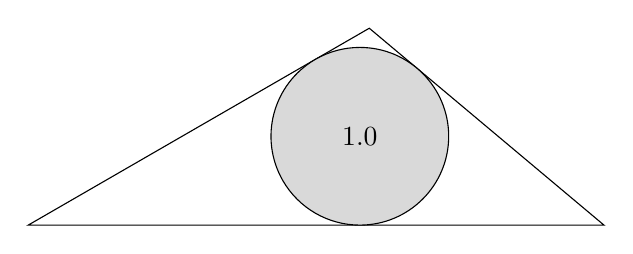
\begin{tikzpicture}[scale=2]
            \hatsinhat{\defaulta}{\defaultb}{0}{0}
        \end{tikzpicture}
        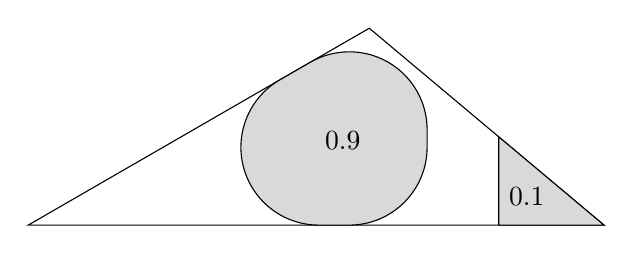
\begin{tikzpicture}[scale=2]
            \hatsinhat{\defaulta}{\defaultb}{0.1}{0}
        \end{tikzpicture}

        \vspace{5mm}

        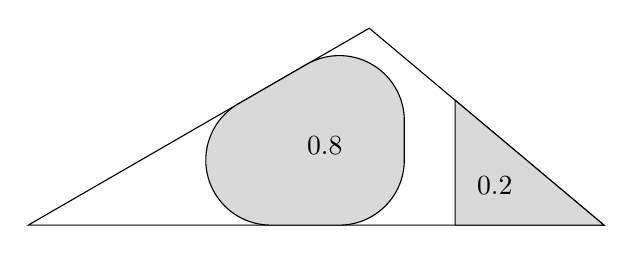
\begin{tikzpicture}[scale=2]
            \hatsinhat{\defaulta}{\defaultb}{0.2}{0}
        \end{tikzpicture}
        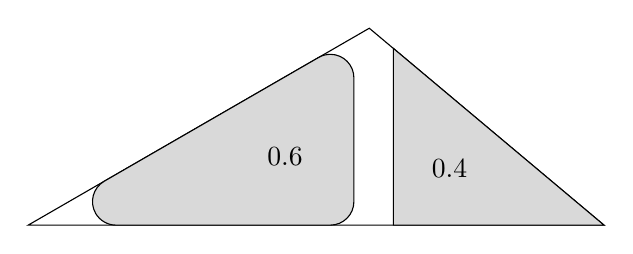
\begin{tikzpicture}[scale=2]
            \hatsinhat{\defaulta}{\defaultb}{0.4}{0}
        \end{tikzpicture}

        \vspace{5mm}

        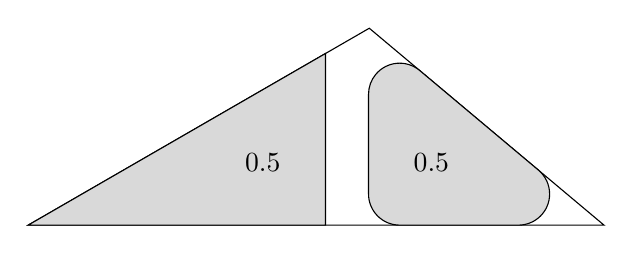
\begin{tikzpicture}[scale=2]
            \hatsinhat{\defaulta}{\defaultb}{0.5}{0}
        \end{tikzpicture}
        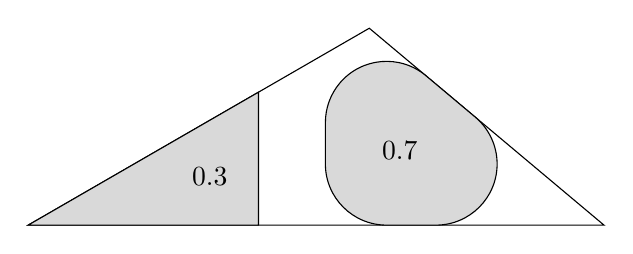
\begin{tikzpicture}[scale=2]
            \hatsinhat{\defaulta}{\defaultb}{0.7}{0}
        \end{tikzpicture}

        \vspace{5mm}

        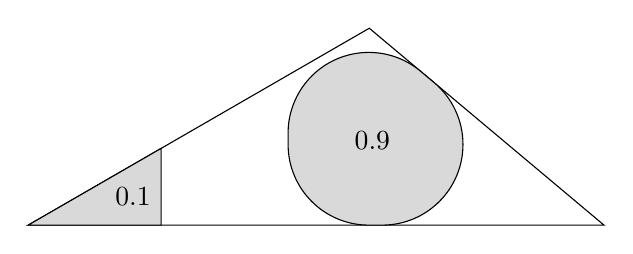
\begin{tikzpicture}[scale=2]
            \hatsinhat{\defaulta}{\defaultb}{0.9}{0}
        \end{tikzpicture}
        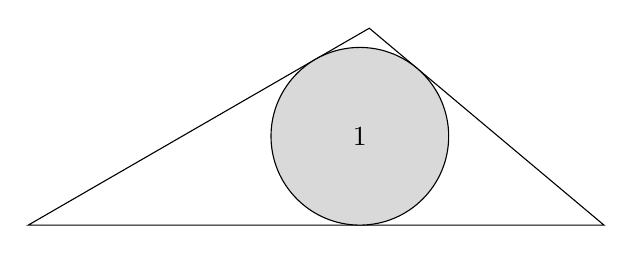
\begin{tikzpicture}[scale=2]
            \hatsinhat{\defaulta}{\defaultb}{1}{0}
        \end{tikzpicture}

        \caption{Hat-in-hat packings for different values of $a_1$ and $a_2$}
        \label{fig:hatsinhat}
    \end{figure}

    This placement constitutes a valid packing if (1) the hats do not overlap each other and (2) the hats fit into the hat individually. We are going to proof these two properties separately.

    \begin{itemize}
        \item[(1)]
            We want to show that the hats do not overlap each other.

            We first normalize the container hat's width to 1 and make an observation about the partial widths $l$ and $r$ in \Cref{fig:hatlr}: If the top angle is a right angle, the partial widths have the same lengths as the triangle's two cathetus $x$ and $y$, so by Pythagoras, $l^2 + r^2 = 1$. If the top angle is more obtuse, but the incircle's center stays at the same $x$-coordinate (like the dotted variant), both $l$ and $r$ shrink, so for each hat, $l^2 + r^2 \le 1$, or $r \le \sqrt{1-l^2}$.

            \begin{figure}[htbp!]
                \centering

                \begin{tikzpicture}[scale=3]
                    \hatlr{\defaulta}{\defaultb}{39}{51}
                \end{tikzpicture}

                \caption{$l^2 + r^2 \le 1$ holds for each non-acute triangle}
                \label{fig:hatlr}
            \end{figure}

            We then observe that the two hats do not overlap if their incircles don not overlap. If we enclose these incircles with hats similar to the container, like in \Cref{fig:hatsoverlap}, we see that they do not overlap if $lf + rg \le w$ holds.

            Also note that for similar hats, the ratio between their incircle's area and the square of their widths is constant. This means that if $a_1 + a_2 \le a$, then $f^2 + g^2 \le w^2$. Thus, $g \le \sqrt{w^2-f^2}$.

            \begin{figure}[htbp!]
                \centering

                \begin{tikzpicture}[scale=3]
                    \hatsoverlap{\defaulta}{\defaultb}{\defaultx}{0}
                \end{tikzpicture}

                \caption{$f^2 + g^2 \le w^2$ for each non-acute triangle}
                \label{fig:hatsoverlap}
            \end{figure}

            Putting it all together, we can show the required property:

            \begin{align*}
                lf + rg
                &\le lf + \sqrt{1-l^2} \sqrt{w^2-f^2}\\
                &= lf + \sqrt{(1-l^2)(w^2-f^2)}\\
                &= lf + \sqrt{w - \textcolor{blue}{l^2w^2} - \textcolor{blue}{f^2} + l^2f^2}\\
                &\le lf + \sqrt{w - \textcolor{orange}{2lwf} + l^2f^2}\tag{\theequation}\label{eq:am-gm}\\
                &= lf + \sqrt{(w-lf)^2}\\
                &= w
            \end{align*}

            Line \ref{eq:am-gm} is a consequence of the inequality of arithmetic and geometric means: $\frac{lw+f}{2} \ge \sqrt{lwf} \Rightarrow \frac{(lw+f)^2}{4} \ge lwf \Rightarrow l^2w^2 + 2 lwf + f^2 \ge 4 lwf \Rightarrow \textcolor{blue}{l^2w^2 + f^2} \ge \textcolor{orange}{2lwf}$.

        \item[(2)]
            The second property we need to show is that the hats fit inside the container individually.

            If a hat's incircle area $a_i < f_i$, its incircle is smaller than the incircle of the container hat's side, so it will fit inside without question (like all the not-rounded hats in \Cref{fig:hatsinhat}).

            So let us assume $a_i \ge f_i$. For this proof, normalize the container hat's incircle to 1. Again, for hats similar to the container hat's right side, the ratio between the square root of its incircle's area and the length of its base is constant. We call this constant $d$.
            %Also, we are interested in the fraction $\frac{x}{d}$ in \Cref{fig:hatpokef}, which specifies “which fraction of the longest side of a triangle similar to the container's right side is above a tangent to its incircle parallel to the container triangle's left side”. We can observe that
            We are also interested in the ratio between the square root of the incircle's area of a triangle similar to the container triangle and the length of its right side. We call this ratio $e$. See \Cref{fig:hatpokef} for an illustration of $d$ and $e$.

            From the same figure we can observe that

            $$e\sqrt{a} = d\sqrt{f_i} \iff e = d\sqrt{\frac{f_i}{a}}$$

            %$$\frac{x}{d} = \frac{d-d\sqrt{f_i})}{d} = 1 - \sqrt{f_i}$$

            \begin{figure}[htbp!]
                \centering

                \begin{tikzpicture}[scale=3]
                    \hatpokef{\defaulta}{\defaultb}{\defaultx}{0}
                \end{tikzpicture}

                \caption{}
                \label{fig:hatpokef}
            \end{figure}

            In \Cref{fig:hatpoke}, we display the situation when packing a hat into the right side of the container. $f_i$ is the relevant factor from the split key, $a_i$ is the hat's incircle and $y$ is a circle which represents the hat's rounding.

            \begin{figure}[htbp!]
                \centering

                \begin{tikzpicture}[scale=3]
                    \hatpoke{\defaulta}{\defaultb}{\defaultx}{0}
                \end{tikzpicture}

                \caption{}
                \label{fig:hatpoke}
            \end{figure}

            The hat is placed in such a way that it will never overlap the bottom or the right side of the containing triangle, so it is sufficient to show that it does not overlap the left side.
            We can tell from \Cref{fig:hatpoke} that this does not happen if the width of the hat's triangle ($d\sqrt{a_i}$), minus the width of the $(y,0)$-triangle similar to the containers right side ($d\sqrt{y}$), plus the length of the right side of the $(y,0)$-triangle similar to the container ($e\sqrt{y}$) is at most the length of the container triangle's right side ($d\sqrt{f_i}$):

            \begin{align*}
                d\sqrt{a_i} - d\sqrt{y} + e\sqrt{y} \le d\sqrt{f_i}\\
            \end{align*}

            We replace $e$ as by the above observation:

            \begin{align*}
                d\sqrt{a_i} - d\sqrt{y} + d\sqrt{\frac{f_i}{a}}\sqrt{y} \le d\sqrt{f_i}\\
            \end{align*}

            And immediately divide by $d$:

            \begin{align*}
                \sqrt{a_i} - (1-\sqrt{f_i})\sqrt{y} \le \sqrt{f_i}
            \end{align*}

            By assumption, the hat is rounded by $y = a_i - f_i\frac{1-a_i}{1-f_i} = \frac{a_i(1-f_i)-f_i(1-a_i)}{1-f_i} = \frac{a_i-f_i}{1-f_i}$.
            Also substitute $f_i = b^2$ and $a_i-f_i = c^2$, and the inequality becomes

            $$\sqrt{b^2+c^2} - (1-b)\frac{c}{\sqrt{1-b^2}} \le b$$

            Bring the subtrahend to the right and square both sides.

            $$b^2+c^2 \le b^2 + \frac{2b(1-b)c}{\sqrt{1-b^2}} + (1-b)^2\frac{c^2}{1-b^2}$$

            Subtract $b^2$, divide by $c$, and rearrange, then multiply with $\sqrt{1-b^2}$:

            $$c\frac{(1-b^2)-(1-b)^2}{\sqrt{1-b^2}} \le \frac{(1-b^2)-(1-b)^2}{\sqrt{1-b^2}}\sqrt{1-b^2}$$

            Divide by the large fraction, and resubstitute:

            \begin{align*}
                &c \le \sqrt{1-b^2}\\
                \iff &c^2 \le 1-b^2\\
                \iff &a_i - f_i \le 1-f_i\\
                \iff &a_i \le 1\\
            \end{align*}

            As $a_i$ is never larger than 1, the original condition is true and the hat always fits into the container.
    \end{itemize}
\end{proof}

\begin{lemma}\label{th:roundedhatsinhat}
    Consider an $(a,b)$-hat with the associated split key $F = (f_1, f_2)$, and call its left- and right-angles $\alpha$ and $\beta$.
    For all $(F,b)$-rounded tuples $(a_1, b_1)$ and $(a_2, b_2)$ with $a_1 + a_2 \le a$, the following two shapes can be packed into the hat:
    \begin{itemize}
        \item A right $(a_1,b_1)$-hat with a right-angle of $\alpha$ and
        \item a right $(a_2,b_2)$-hat with a left-angle of $\beta$.
    \end{itemize}
\end{lemma}

\begin{proof}
    \Cref{th:hatsinhat} tells us that this theorem is true for $b = 0$. Now, the container's corners can be rounded to the radius of a $b$-circle, and we need to show that the two hats from the previous construction still fit inside. But all of the two hat's corners are also rounded to (at least) the same radius, so they will never overlap the container, see \Cref{fig:rounding-hats}.
\end{proof}

\begin{figure}[htbp!]
    \centering

    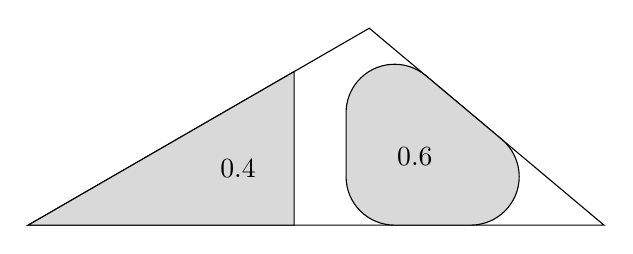
\begin{tikzpicture}[scale=2]
        \hatsinhat{\defaulta}{\defaultb}{\defaultx}{0}
    \end{tikzpicture}
    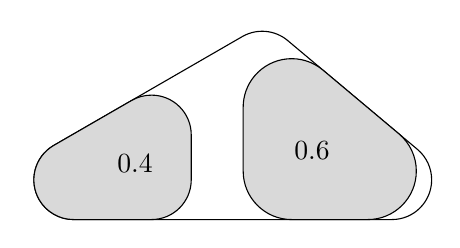
\begin{tikzpicture}[scale=2]
        \hatsinhat{\defaulta}{\defaultb}{\defaultx}{\defaultr}
    \end{tikzpicture}

    \caption{Rounding all hats' corners by the same radius does not affect the packing.}
    \label{fig:rounding-hats}
\end{figure}

\begin{theorem}
    Each $(a,b)$-hat is a $\C(a,b)$-shape.
\end{theorem}

\begin{proof}
    \Cref{def:hat-split-key} tells us how to compute the split key $F$.

    We proof by induction that we can pack each $c \in \C(a,b)$ into the hat:

    If $c$ only consists of a single $a_1$-circle it can be packed into the hat, as it is as most as big as the hat's incircle of area $a$.

    Assume that for each $(a,b)$-hat, all instances in $\C(a,b)$ with at most $n$ circles can be packed. Consider an instance $c$ containing $n+1$ circles. Then we know from \Cref{th:split-rounded} that \textsc{Split} will partition $c$ into two subinstances

    \Cref{th:roundedhatsinhat} tells us how to determine two shapes which always fit into the hat. It's left to show that these shapes are $(F,b)$-rounded. We proceed by induction:

    and \Cref{th:split-rounded}, it follows directly that the hat is a $\C(a,b)$-shape.
\end{proof}

\section{Triangles}

\begin{theorem}
    For any non-acute triangle with an incircle of area $a$, for any $b > a$ there are instances in $\C(b)$ which cannot be packed into the triangle.
\end{theorem}

\begin{proof}
    The instance $\{b\}$ cannot be packed, as the incircle is by definition the largest circle which fits into the triangle.
\end{proof}

\begin{theorem}
    A non-acute triangle with an incircle of area $a$ is a $\C(a)$-shape.
\end{theorem}

\begin{proof}
    The triangle is an $(a,0)$-hat, which is a $\C(a)$-shape.
\end{proof}

%\begin{theorem}
%    Each $A \in \C(a)$ can be packed into an isosceles triangle with a largest angle $\gamma$ between $\frac{\pi}{2}$ and $\frac{\pi}{3}$ and an area of $a\frac{1+\frac{1}{\sin(\gamma)}}{\pi}$.
%\end{theorem}
%
%\begin{theorem}
%    For any $0 < x$ and $0 < y$, there are always 
%    a $(x+z)$-hat and a
%    Each $A \in \C(a)$ can be packed into an obtuse triangle with an incircle of area $a$.
%\end{theorem}
%
%\chapter{Squares}
%
%\begin{figure}[htbp!]
%    \centering
%
%    \begin{tikzpicture}[scale=2]
%        \hatsinsquare{0.5}
%    \end{tikzpicture}
%    \begin{tikzpicture}[scale=2]
%        \hatsinsquare{0.49}
%    \end{tikzpicture}
%    \begin{tikzpicture}[scale=2]
%        \hatsinsquare{0.4}
%    \end{tikzpicture}
%    \begin{tikzpicture}[scale=2]
%        \hatsinsquare{0.2}
%    \end{tikzpicture}
%    \begin{tikzpicture}[scale=2]
%        \hatsinsquare{0}
%    \end{tikzpicture}
%
%    \caption{Hat-in-square packings for different values of $\frac{x}{x+y}$}
%    \label{fig:hatsinsquare}
%\end{figure}
%
%
%
%Finally, we can bring the \textsc{Split} algorithm and the properties of the hat shapes together and give constructive proofs for the existence of circle packings:

%\begin{proof}
%Call the hat's smaller angles $\alpha$ and $\beta$. Set $f = $
%\end{proof}
%
%We are now ready to prove our main theorem:
%

\section{Squares}

\begin{lemma}
    If the circle instance shown in \Cref{fig:b} has a combined area of $a$, the square has an area of $\frac{3+2\s}{\pi}a \approx 1.85525a$. Call this worst-case factor $\Psi$.
\end{lemma}

\begin{proof}
    Note that because a circle of radius $r$ has an area of $a = \pi r^2$, an $a$-circle has a radius of $r = \sqrt{\frac a \pi}$. Then, by construction as seen in \Cref{fig:b}:

    $$\Psi a = \left(2r + 2\frac{r}{\s}\right)^2 = r^2\left(2+\s\right)^2 = \frac{\frac a 2}{\pi}\left(4+4\s+2\right) = \frac{3+2\s}{\pi}a$$
\end{proof}

\begin{figure}[htbp!]
    \centering

    \begin{tikzpicture}[scale=3]
        \squareworstcaseconstruction
    \end{tikzpicture}

    \caption{Constructing $\Psi$.}
    \label{fig:b}
\end{figure}

Our problem can now be expressed like this: Can all circle instances $A \in \C(a)$ be packed into a square with an area of $\Psi a$? This will be \Cref{th:circlesinsquare}, and the rest of this paper will build up to its proof.


\begin{theorem}\label{th:circlesinsquare}
    A square with an area of $\frac{3+2\s}{\pi} a$ is a $\C(a)$-shape.
\end{theorem}

%\begin{theorem}\label{th:hatsinsquare}
%    For any $0 \le x \le y$, an $x$-hat and a $(y,y-x)$-hat can always be packed into a square with an area of $\Psi(x+y)$.
%\end{theorem}
%
%\begin{proof}
%    Place the tips of the hats in two opposing corners of the square, like in \Cref{fig:hatsinsquare}.
%    This placement constitues a valid packing if (1) the hats fit into the square individually and (2) the hats do not overlap.
%
%    \begin{itemize}
%        \item[(1)]
%            The hats fit into the square individually if their diagonal never gets larger than the square's edge length $\sqrt{\Psi(x+y)} = \frac{1+\s}{\sqrt{\pi}}\sqrt{x+y}$.
%            As $x \le \frac {x+y} 2$, \Cref{lm:sizes} directly tells us that the $x$-hat has a diagonal of at most
%            \begin{align*}
%                d(x,0) \le d(\frac{x+y}{2},0) = \sqrt{\frac{\frac{x+y}{2}}{\pi}}(2+\s) + 0 = \sqrt{\Psi(x+y)}
%            \end{align*}
%
%            As for the $(y,y-x)$-hat, its diagonal is also never larger than $\sqrt{\Psi(x+y)}$: \todo[inline]{algebraic proof TBD :-)}
%
%            \begin{tikzpicture}
%                \begin{axis}[height=5cm,xtick={0,0.5},xlabel=$\frac{x}{x+y}$,domain=0:0.5,legend pos=outer north east,no markers,samples=500]
%                    \addplot[red,thick] {sqrt((1-x)/pi)*(2+sqrt(2))-sqrt((1-2*x)/pi)*sqrt(2)};
%                    \addplot[blue,thick] {(1+sqrt(2))/sqrt(pi)};
%                    \legend{$\frac{d{(y,y-x)}}{\sqrt{x+y}}$,$\sqrt{\Psi}$}
%                \end{axis} 
%            \end{tikzpicture}
%
%            %\begin{align*}
%            %    d(y,y-x)
%            %    &= \sqrt{\frac{y}{\pi}}(2+\s)-\sqrt{\frac{y-x}{\pi}}\s\\
%            %    &\le \sqrt{\frac{\frac{x+y}{2}}{\pi}}(2+\s)-\sqrt{\frac{y-y}{\pi}}\s\\
%            %    &= \frac{1+\s}{\sqrt{\pi}}\sqrt{x+y} = \sqrt{\Psi(x+y)}
%            %\end{align*}
%
%        \item[(2)]
%            The hats don't overlap if their combined height never exceeds $\sqrt{2\Psi(x+y)}$, the square's diagonal:
%            \begin{align*}
%                h(x) + h(y)
%                &= \sqrt{\frac{x}{\pi}}(1+\s) + \sqrt{\frac{y}{\pi}}(1+\s)\\
%                &= \frac{1+\s}{\sqrt\pi}(\sqrt{x}+\sqrt{y})\\
%                &\le \frac{1+\s}{\sqrt\pi}(\sqrt{2x+2y})\\
%                &= \s\frac{1+\s}{\sqrt\pi}\sqrt{x+y} = \sqrt{2\Psi(x+y)} \qedhere
%            \end{align*}
%    \end{itemize}
%\end{proof}

%\begin{proof}
%    If $A$ only consists of a single $a$-circle, it can be placed at the center of the square, as its diameter of $2\sqrt{\frac{a}{\pi}} \approx 1.12838\sqrt{a}$ is smaller than the squares edge length $\sqrt{\Psi a} \approx 1.36207\sqrt{a}$. Otherwise, by \Cref{th:split-property}, \textsc{Split} decomposes $A$ into $X \in \C(x)$ and $Y \in \C(y,y-x)$. By \Cref{th:circlesinhat}, we can pack $X$ into a $x$-hat and $Y$ into a $(y,y-x)$-hat. By \Cref{th:hatsinsquare}, we can pack those two hats into the square.
%
%    See \Cref{fig:example} for a complete example packing.
%\end{proof}
%
%\begin{figure}[htbp!]
%    \centering
%    \includegraphics[width=0.5\textwidth]{square_example.png}
%    \caption{Packing of an example instance.}
%    \label{fig:example}
%\end{figure}

\chapter{Conclusions and Future Work}

\appendix

\end{document}
